%\documentclass[]{spie}  %>>> use for US letter paper
\documentclass[a4paper,nocompress]{spie}  %>>> use this instead for A4 paper
%\documentclass[nocompress]{spie}  %>>> to avoid compression of citations

\renewcommand{\baselinestretch}{1.0} % Change to 1.65 for double spacing
 
\usepackage{amsmath,amsfonts,amssymb}
\usepackage{graphicx}
\usepackage[colorlinks=true, allcolors=blue]{hyperref}
\usepackage[dvipsnames]{xcolor}
\usepackage{tabularx}
\setlength{\extrarowheight}{2pt}

\title{Quantifying the Impact \\ of Performance Improvements and Cost Reductions \\ from 20 years of Light-Emitting Diode Manufacturing}

\author[a,b]{Michael Weinold}
\author[b]{Sergey Kolesnikov}
\author[c]{Laura Diaz Anadon}
\affil[a]{ETH Zurich, Chair of Entrepreneurial Risks, Scheuchzerstrasse 7, 8092 Zurich, Switzerland}
\affil[b]{University of Cambridge, Centre for Environment, Energy and Natural Resource Governance, The David Attenborough Building, CB2 3QZ Cambridge, UK}

\authorinfo{Further author information: (Send correspondence to Michael Weinold)\\Michael Weinold: E-mail: michael.weinold@alumni.ethz.ch}

% Option to view page numbers
\pagestyle{empty} % change to \pagestyle{plain} for page numbers   
\setcounter{page}{301} % Set start page numbering at e.g. 301
 
\begin{document} 
\maketitle

\begin{abstract}
We collected historical data on device performance, technological breakthroughs and manufacturing innovation for phosphor-converted white light-emitting diodes for the past 20 years. We used this information to identify and quantify the principal sources of performance improvements in LED manufacturing. We found that in order to quantify the impact of single technological changes, it is necessary to analyse performance improvements the device sub-efficiency level. We further developed a bottom-up manufacturing cost model with process step resolution that captures improvements in throughput, yield and related costs of all relevant manufacturing steps, as well as economies of scale to analyse cost reductions and their sources. It covers progress from early manufacturing in 2003 to today. We found that larger wafer sizes have been largely responsible for cost reductions. We found that XXX well known XXX.

\end{abstract}

% Include a list of keywords after the abstract 
\keywords{light-emitting diodes, innovation, efficiency, cost}

\section{INTRODUCTION}
\label{sec:intro}  % \label{} allows reference to this section

\clearpage
\section{METRICS}


However, the total flux per die is 

\begin{figure} [ht]
    \begin{center}
        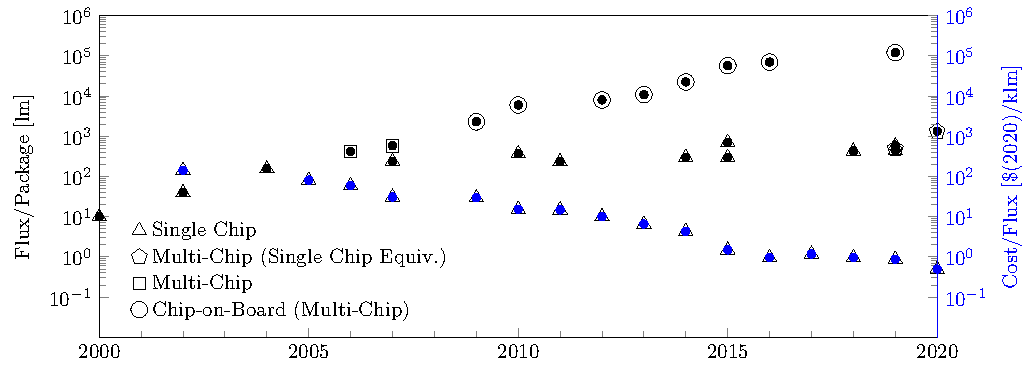
\includegraphics[width=\textwidth]{haitz_law_white.pdf}
    \end{center}
    \caption{Historical increase in flux for white light-emitting diode chips and packages, inspired by \textit{"Haitz's Law"}. Note that the increase in flux per single chip is not increasing as starkly as the flux for multi-chip packages. Shown are datapoints for best commercial performers from press releases, datasheets and and industry periodicals.}
\end{figure} 
    
Mention previous work by Tsao et al.
Mention limitations: Not done for 2003 (early devices) and 2020 (most recent devices)

The overall efficiency of a light-emitting diode is the product of the sub-efficiencies associated with an ensemble of different loss channels. Sub-efficiencies directly capture the effect of technology breakthroughs in device design and manufacturing process improvements. They thus provide the best metric to quantify technology breakthroughs.


        It describes the electrical and optical losses within the device, as well as the conversion losses in the phosphor layer. It further considers the mismatch between the device spectrum and an optimal spectrum, accounting for the wavelength dependent sensitivity of the human eye.

    \begin{table}[h!]
        \caption{List of the device sub-efficiencies used in our methodology. We follow the definitions used by previous authors, such as Tsao et al. \cite{tsao2010solid} and Pattison et al. \cite{pattison2017solid}. The historical development of the sub-efficiencies is displayed in figure \ref{fig:efficiency}. *Also called "lamp efficiency" or "cumulative efficiency" by authors, such as Tsao et al. \cite{tsao2010solid}}
        \bigskip
        \centering
    	\begin{tabularx}{\textwidth}{|l|l|l|X|}
    		\hline
    			\textit{Symbol} & \textit{Sub-Efficiency} & \textit{Loss-Channel} & \textit{Definition} \\
    		\hline
    		    $\eta_{V_f}$ & Forward Voltage Efficiency* & Ohmic Resistance & $\eta_{V_f} = E_{h\nu} / V_f $ \\
    		\hline
    		    $\eta_{LE}$ & Light-Extraction Efficiency & Re-absorption and Reflection & $\eta_{LE}= P_{out} / P_{in} $ \\
    		\hline
    		    $\eta_{IQ}$ & Internal Quantum Efficiency & Non-radiative Recombinations & $\eta_{EQ} = \eta_{IQ} \times \eta_{LE}$ \\
    		\hline
    		    $\eta_{Droop}$ & (Electrical) Droop & Non-radiative Recombinations & $\eta_{Droop} = 1 - \eta_{IQE} / \eta_{IQE}(A \rightarrow 0) $ \\
    		\hline
    		    $\eta_C$ & Conversion Efficiency & Stokes Loss, Absorption, etc. & $\eta_{C} = E_{\textcolor{blue}{B}} / \sum_{i=\textcolor{red}{R},\textcolor{orange}{O},\textcolor{yellow}{Y},\textcolor{teal}{G}} E_i$ \\
    		\hline
    		    $\eta_{S}$ & Spectral Efficiency & Eye Sensitivity & $\eta_{S} = K / K_{max}(CRI,CCT)$ \\
    		\hline
    		    $\eta_L$ & Lamp Efficiency & N/A (Cumulative) & $\eta_L = \prod_{i=(V_f,\dots,S)} \eta_i$ \\
            \hline
                \multicolumn{4}{|l|}{$\!\begin{aligned}
                    E_{h\nu} &\dots \text{photon energy} \\
                    V_f &\dots \text{forward voltage} \\
                    A &\dots \text{electrical current} \\
                    E_{B,\dots,G} &\dots \text{optical energy of monochromatic light (blue, red, orange, yellow, green)} \\
                    K &\dots \text{luminous efficacy of radiation} \\
                    CRI &\dots \text{color rendering index}, \ CCT \dots \text{color temperature} \\
                \end{aligned}$} \\
            \hline
    	\end{tabularx}
    \end{table}


\clearpage

\section{METHODS}
\label{sec:methods}

To quantify changes in the manufacturing cost of devices, a bottom-up manufacturing cost model with process step resolution was constructed to cover the entire manufacturing process of GaN-on-sapphire based phosphor converted low-to-mid power light-emitting diode packages of different chip architectures. We considered classical p-side-up lateral current spreading devices, as well as a packaged flip-chip vertical current spreading architecture and a chip-scale package flip chip architecture. The model was constructed for the years 2003, 2012 and 2020. It was populated with equipment data from European and North American firms, selected for a virtual North American manufacturing location. Process specific step parameters were derived from scientific literature, company publications, archived product catalogs and patent literature. Details of the manufacturing process, as well as changes in the same were gathered from detailed patent analysis, augmented by interviews with experts from industry and academia. For 2012, data for the model was adapted from the \textit{LEDCOM} cost model prepared for the US Department of Energy by Stephen Bland. The model includes both the wafer treatment process as well as the packaging process. It is important to note that the aim of the model is not to faithfully represent real world manufacturing conditions in Asia based plants, but rather to show the effect of single technological changes in the manufacturing process on total cost. This means that while the model does consider overhead costs and depreciation, it does so only to XXXX 

Also to diagreggate contribution of single changes
To dis-aggregate the contribution of changes in manufacturing process steps to total manufacturing cost, we used an approach introduced by Kavlak et al. in a cost model with similar process step resolution for solar photovoltaics. It is based on the logarithmic derivative of the total differential of the cost function.

Equation here

To gain a detailed understanding of the sources and magnitude of efficiency improvements in devices, we gathered data on overall device performance and identified the associated device architecture and types of down conversion phosphors used. We systematically identified the improvements related to each device sub-efficiency, gathered associated efficiency data from literature or computed the respective values from raw data.
For instance, in the case of spectral efficiency and the performance related to consumer experience metrics, we identified the prevalent red and yellow phosphors used during the period of interest. We then computed luminous efficacy of radiation as well as the color rendering index and color temperature from the spectral data. The development history of each phosphor was researched to determine if it had been developed specifically for use in light emitting devices, or if it was instead the result of a knowledge spillover.


figure: chip architectures
\begin{figure} [ht]
    \begin{center}
        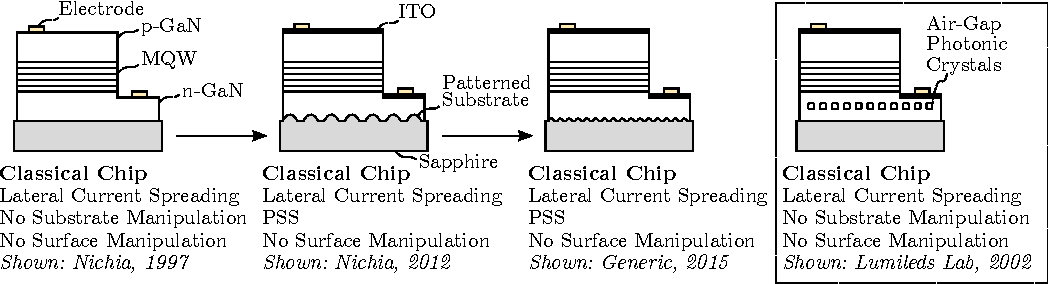
\includegraphics[width=\textwidth]{SPIE/article/chip_architectures.pdf}
    \end{center}
    \caption{Cutaway side views of the evolution of chip architectures for classical chip designs (lateral current spreading). Note that dimensions are not to scale and smaller features are greatly exaggerated for visibility. Years correspond to earliest identified patent priority date. Dashed boxes indicate chip designs not brought to large scale production.}
    \label{fig:chip_arch}
\end{figure}

\begin{figure} [ht]
    \begin{center}
        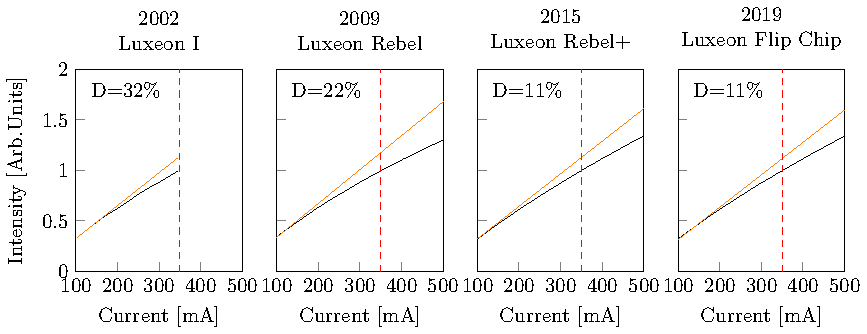
\includegraphics[width=0.85\textwidth]{SPIE/article/droop_lumileds.pdf}
    \end{center}
    \caption{Luminous intensity of four different \textit{Lumileds} high-power light-emitting diodes normalized to the value at a test current of $A_{test}=350$mA. The black curves describe the real measured intensity, the orange curves describe the estimated ideal intensity. Droop is the difference between these curves at the test current. Sources for real curves: XXX}
    \label{fig:chip_arch}
\end{figure}

\section{PERFORMANCE IMPROVEMENTS}

\begin{figure} [ht]
    \begin{center}
        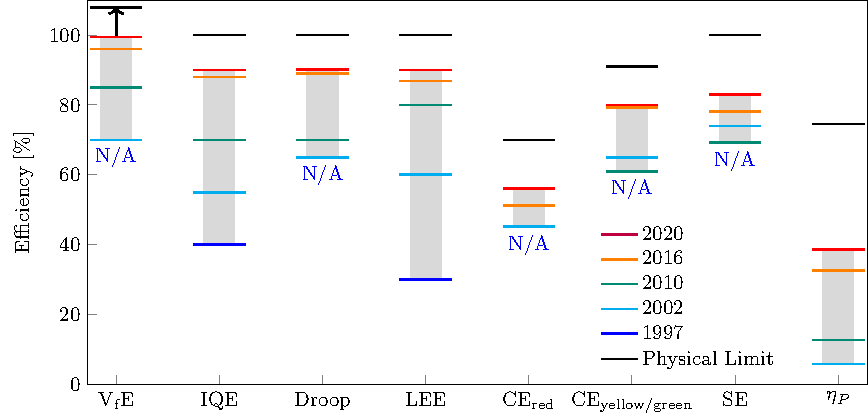
\includegraphics[width=0.85\textwidth]{SPIE/article/breakthroughs_efficiency.pdf}
    \end{center}
    \caption{Impact of technology breakthroughs and manufacturing process improvements on historical improvements in sub-efficiencies of phosphor-converted warm white light-emitting diodes with test currents of at least $I_\text{test}=350$mA. The overall lamp efficiency $\eta_L$ is displayed as the rightmost column. This figure takes as inputs the state-of-the-art sub-efficiencies discussed in section \ref{sec:methods}. Horizontal colored bars give state-of-the-art sub-efficiencies for five years: \textcolor{blue}{1997}, \textcolor{teal}{2002}, \textcolor{orange}{2010}, \textcolor{magenta}{2016} and \textcolor{red}{2020}. Colored annotation "N/A" indicates the sub-efficiency of the corresponding year cannot be computed for the following reasons: V$_\text{f}$E, Droop: depend on current, which was below 350mA at the time; CE, SE: warm white spectrum LEDs not available at the time. Physical limits are indicated by black horizontal bars. The possible range for the physical limit of V$_\text{f}$E exceeds 100\% and depends on electrical device parameters, which are discussed in \cite{david2016electrical}. The range is given by an upward pointing black arrow. Color of vertical bars indicates improvement through either technology spillovers or other improvements (technology breakthroughs or process learning). Spillovers are annotated and listed in an inset table. Efficiency acronyms: forward voltage efficiency (V$_\text{f}$E), internal quantum efficiency (IQE), light extraction efficiency (LEE), conversion efficiency (CE), spectral efficiency (SE), power conversion efficiency ($\eta_{PC}$). Spillover acronyms: patterned sapphire substrate (PSS), indium tin oxide (ITO). Sources: Data for sub efficiencies from figures XXX. Data for XXX.}
    \label{fig:efficiency}
\end{figure}

\subsection{Physical Efficiency}

give two waterfall diagrams (2003,2020) and give one example
example: maybe droop with associated figure. is good example of process improvements

\subsection{Consumer Experience}

List phosphors, give a short overview but do not include figures
show cct spectrum with lines of YAG and 258+ phosphors

\section{MANUFACTURING COST}

show two waterfall diagrams (2003 only). mention work in progress




\acknowledgments % equivalent to \section*{ACKNOWLEDGMENTS}       
 
The main author gratefully acknowledged funding by the \textit{Swiss Study Foundation} of Zurich, Switzerland. The authors further gratefully acknowledge project funding by the \textit{Alfred P. Sloan Foundation} of New York, USA. Cooperation by \textit{Stiftung Warentest} of Berlin, Germany in granting access to their publication archive is gratefully acknowledged.

% References
\bibliography{report} % bibliography data in report.bib
\bibliographystyle{spiebib} % makes bibtex use spiebib.bst

\end{document} 
